\documentclass{article}
\usepackage{cmap}
\usepackage[utf8]{inputenc}
\usepackage[english,ukrainian]{babel}
\usepackage{graphicx}
\usepackage{geometry}
\usepackage{listings}
\usepackage{float}
\usepackage{bm}
\usepackage{amsmath}
\usepackage{pdflscape}
\geometry{
	a4paper,
	left=20mm,
	right=20mm,
	top=20mm,
	bottom=20mm
}
\lstset{
	language=c,
	tabsize=4,
	keepspaces,
	showstringspaces=false,
}
\graphicspath{ {./pictures} }
\setlength{\parindent}{4em}

\newcommand\subject{Архітектура комп'ютера}
\newcommand\lecturer{доцент кафедри ПЗ\\Крук О.Г.}
\newcommand\teacher{доцент кафедри ПЗ\\Крук О.Г.}
\newcommand\mygroup{ПЗ-22}
\newcommand\lab{1}
\newcommand\theme{}
\newcommand\purpose{}

\begin{document}
\begin{normalsize}
	\begin{titlepage}
		\thispagestyle{empty}
		\begin{center}
			\textbf{МІНІСТЕРСТВО ОСВІТИ І НАУКИ УКРАЇНИ\\
				НАЦІОНАЛЬНИЙ УНІВЕРСИТЕТ "ЛЬВІВСЬКА ПОЛІТЕХНІКА"}
		\end{center}
		\begin{flushright}
			Інститут \textbf{КНІТ}\\
			Кафедра \textbf{ПЗ}
		\end{flushright}
		\vspace{200pt}
		\begin{center}
			\textbf{ЗВІТ}\\
			\vspace{10pt}
			До розрахункової роботи № \lab\\
			\textbf{З дисципліни}: “\subject”
		\end{center}
		\vspace{112pt}
		\begin{flushright}
			
			\textbf{Лектор}:\\
			\lecturer\\
			\vspace{28pt}
			\textbf{Виконав}:\\
			
			студент групи \mygroup\\
			Коваленко Д.М.\\
			\vspace{28pt}
			\textbf{Прийняла}:\\
			
			\teacher\\
			
			\vspace{28pt}
			«\rule{1cm}{0.15mm}» \rule{1.5cm}{0.15mm} 2022 р.\\
			$\sum$ = \rule{1cm}{0.15mm}……………\\
			
		\end{flushright}
		\vspace{\fill}
		\begin{center}
			\textbf{Львів — 2022}
		\end{center}
	\end{titlepage}

	\section*{Індивідуальне завданя}
	\begin{figure}[H]
		\centering
		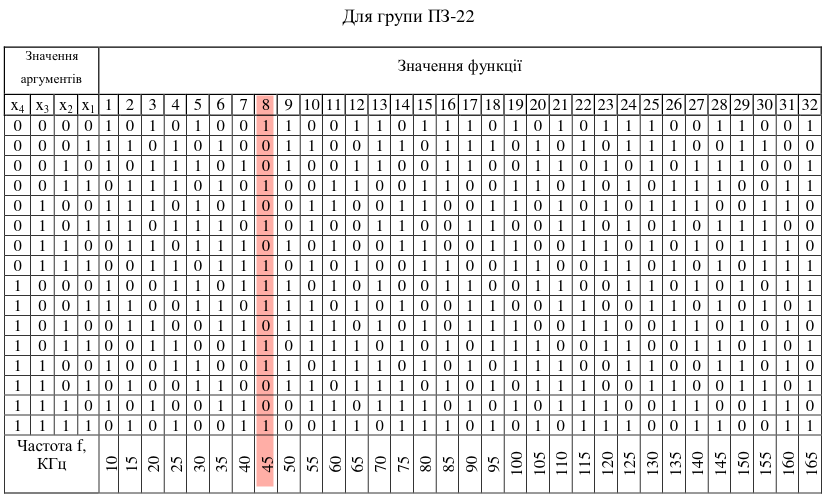
\includegraphics[scale=0.8]{v}
	\end{figure}

	\section*{Хід роботи}
	\subsection*{ДДНФ:}
	\begin{Large}
		\begin{gather}
			\overline{x_4x_3x_2x_1}+\overline{x_4x_3}x_2x_1+\overline{x_4}x_3\overline{x_2}x_1+\nonumber\\
			+\overline{x_4}x_3x_2x_1+x_4\overline{x_3x_2x_1}+x_4\overline{x_3x_2}x_1+\nonumber\\
			+x_4\overline{x_3}x_2x_1+
			x_4x_3\overline{x_2x_1}+
			x_4x_3x_2x_1\nonumber
		\end{gather}
	\end{Large}
	
	\subsection*{Карта Карно}
	\begin{figure}[H]
		\centering
		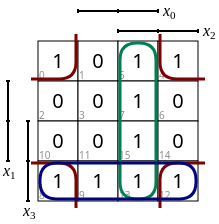
\includegraphics[scale=0.7]{r1}
		\caption{Карта Карно}
	\end{figure}

	\subsection*{$\bm{F_{min1}}$}
	\begin{Large}
		\begin{gather}
			x_2x_1+\overline{x_3x_2x_1}+\overline{x_4}x_3x_1+x_4\overline{x_2x_1}+x_4\overline{x_3x_2}\nonumber
		\end{gather}
	\end{Large}

	\subsection*{Квайна - Мак-Класкі}
	\begin{figure}[H]
		\centering
		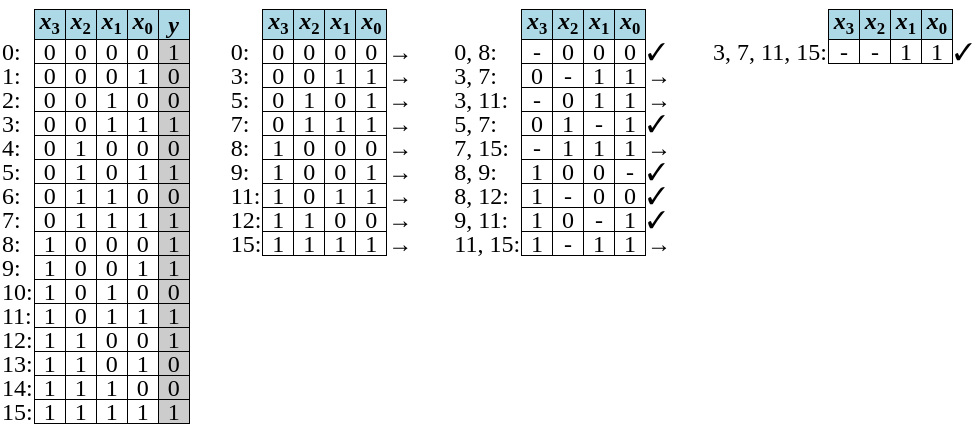
\includegraphics[scale=0.52]{r2}
		\caption{Квайна - Мак-Класкі}
	\end{figure}

	\subsection*{$\bm{F_{min2}}$}
	\begin{Large}
		\begin{gather}
			\overline{x_3x_2x_1}+x_2x_1+\overline{x_4}x_3x_1+x_3\overline{x_2x_1}+x_4\overline{x_3x_2}\nonumber		
		\end{gather}
	\end{Large}

	\subsection*{ДКНФ} 
	\begin{Large}
		\begin{gather}
			(x_4+x_3+x_2+\overline{x_1})
			(x_4+x_3+\overline{x_2}+x_1)
			(x_4+\overline{x_3}+x_2+x_1)\nonumber\\
			(x_4+\overline{x_3}+\overline{x_2}+x_1)
			(\overline{x_4}+x_3+\overline{x_2}+x_1)
			(\overline{x_4}+\overline{x_3}+x_2+\overline{x_1})\nonumber\\
			(\overline{x_4}+\overline{x_3}+\overline{x_2}+x_1)\nonumber
		\end{gather}
	\end{Large}
	
	\section*{Результат роботи}
	\begin{landscape}
		\thispagestyle{empty}
		\begin{figure}[p]
			\vspace*{-2cm}
			\makebox[\linewidth]{
				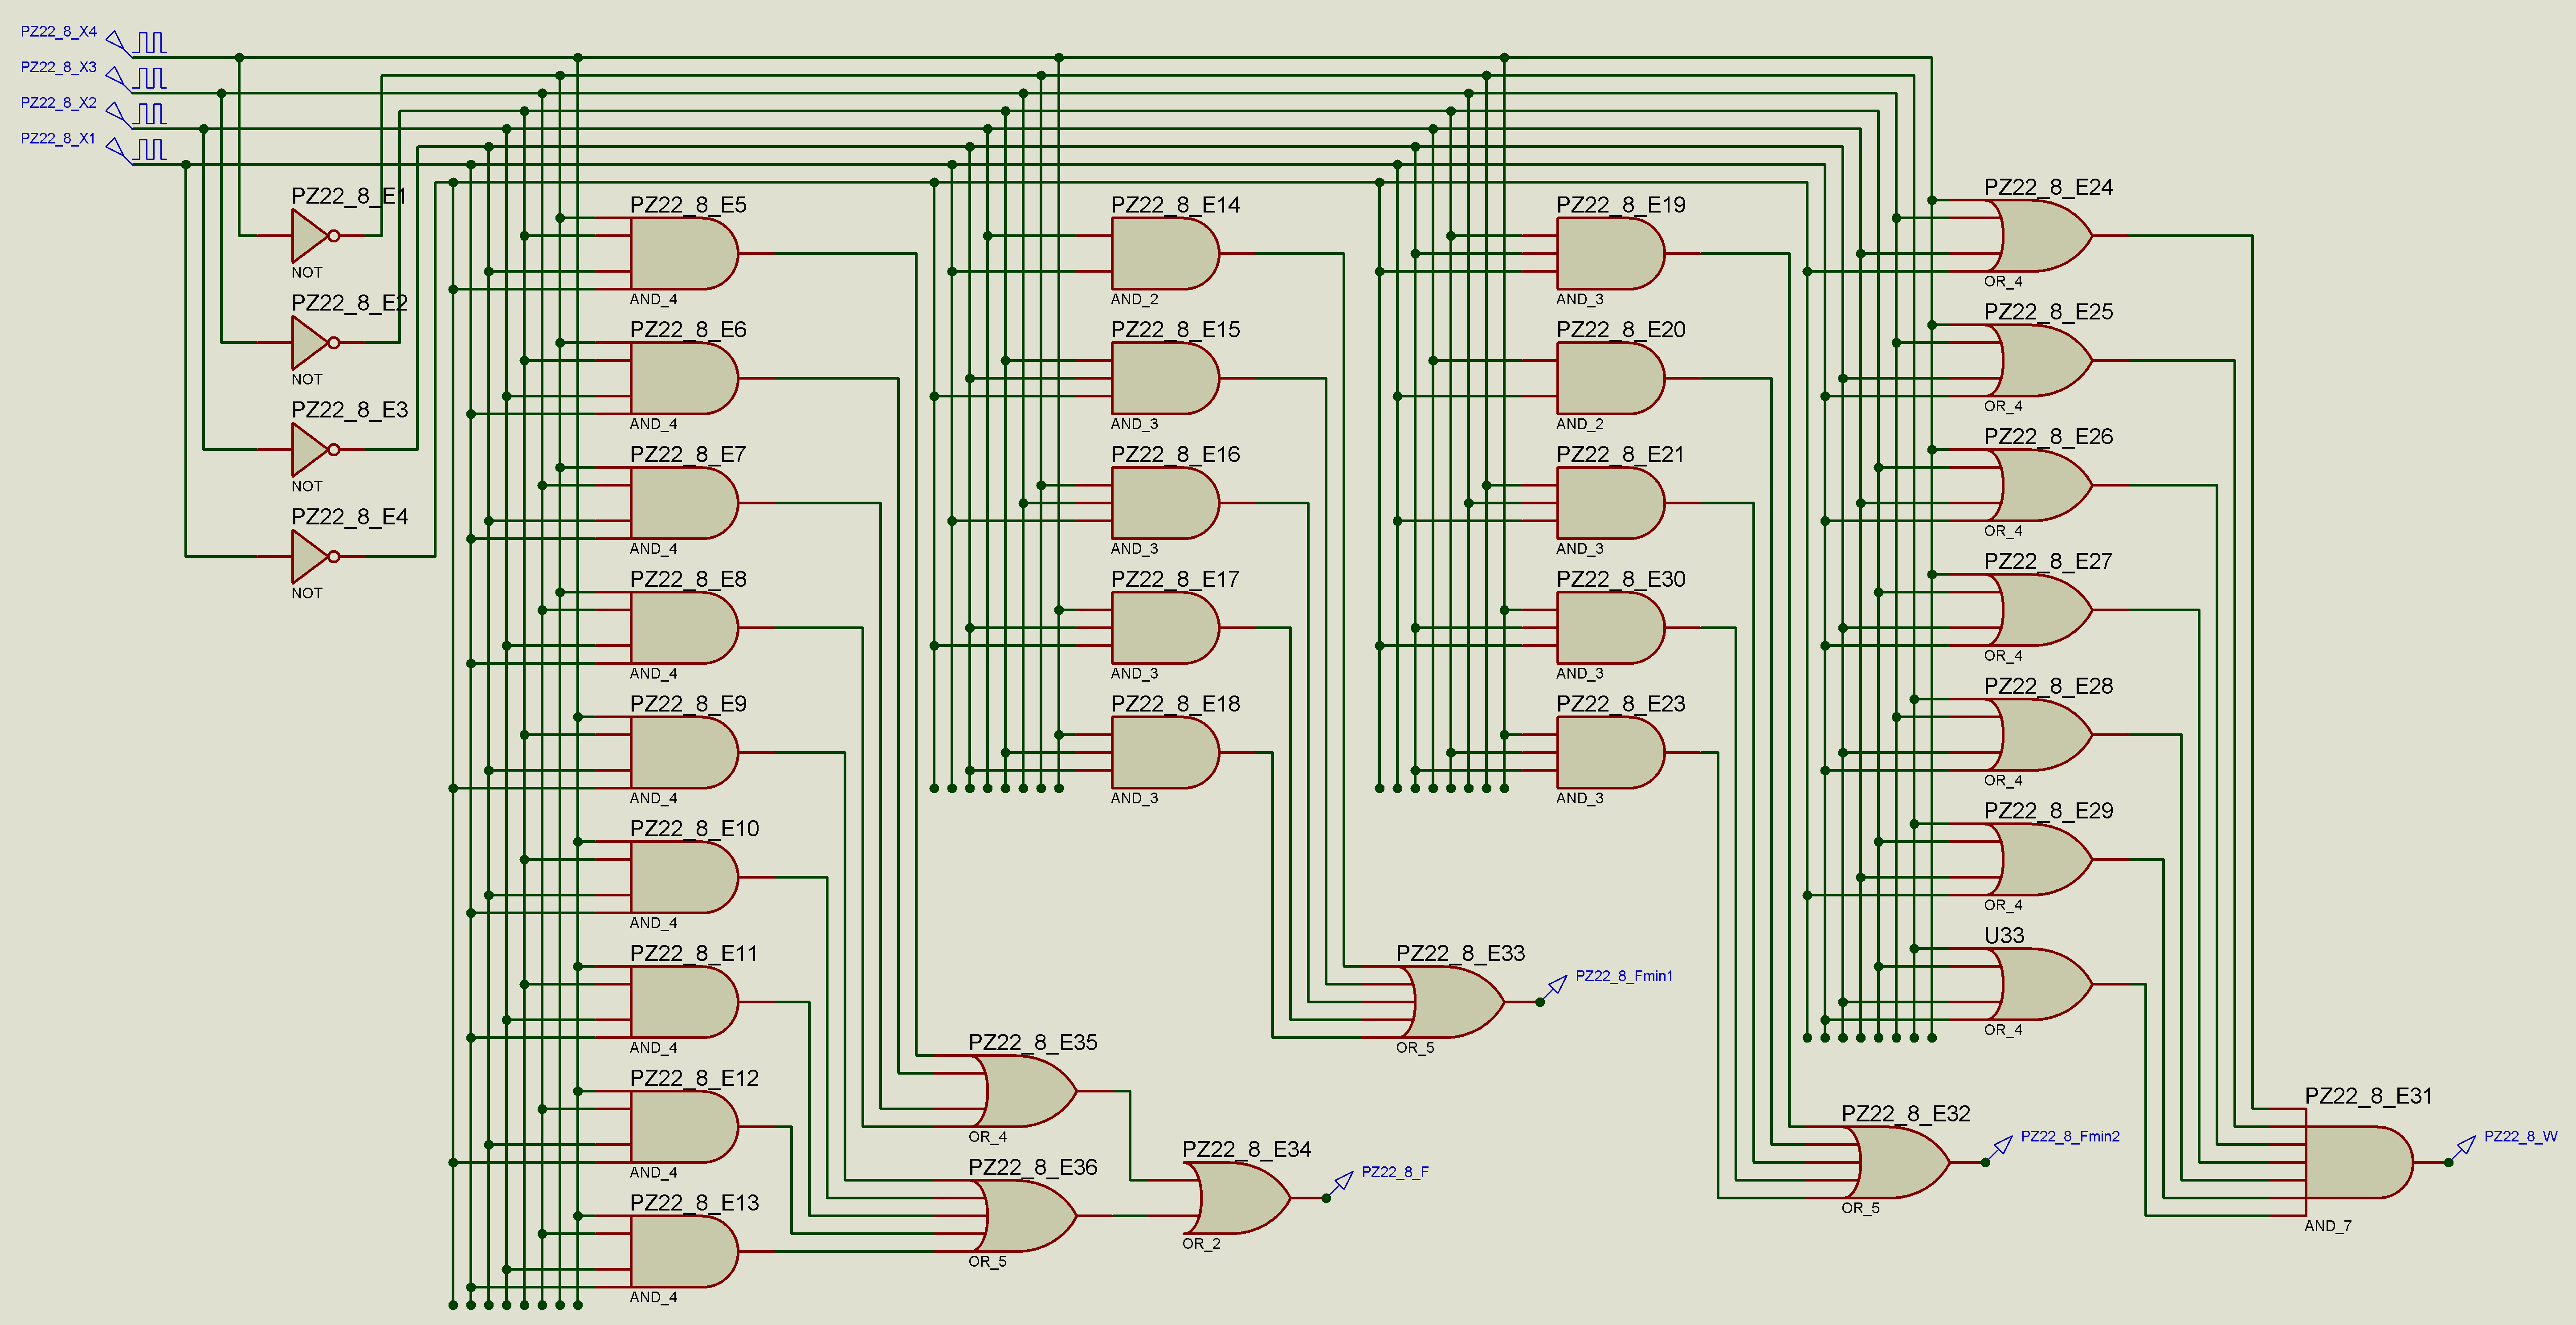
\includegraphics[width=1.15\linewidth]{s}
			}
		\end{figure}
	\end{landscape}

	\begin{figure}[H]
		\centering
		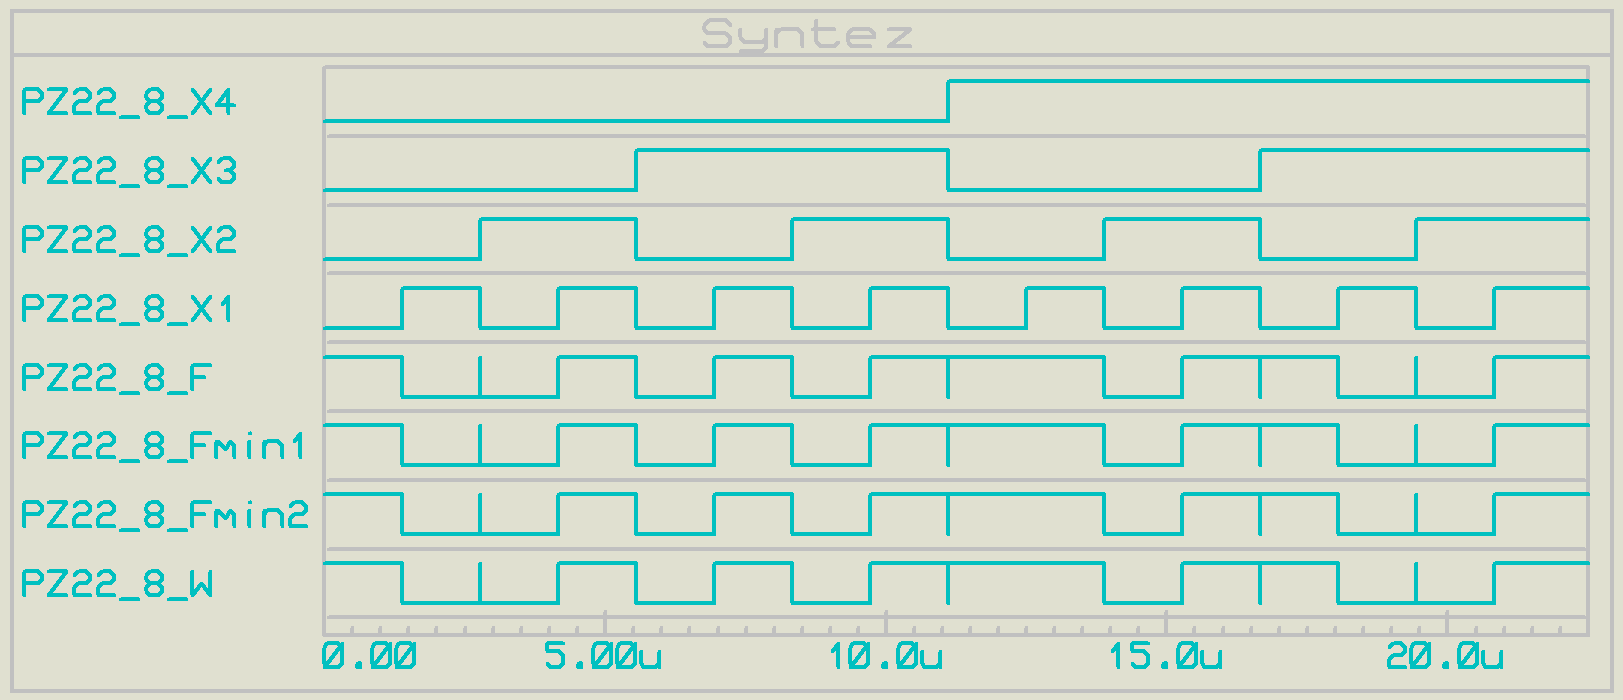
\includegraphics[scale=0.3]{g}
		\caption{Графік "Syntez".}
	\end{figure}
	    
\end{normalsize}
\end{document}
